\chapter{Virtual Private Network (VPN)}
\begin{itemize}
\item We use Soft-Ether Virtual Private network in order to provide secure connection to other network over internet
\end{itemize}
Unfortunately, our administrator, who currently works at home, needs unrestricted remote access to the servers. Since we do not want to get rid of our security improvements, we setup a VPN to achieve that goal.
\begin{figure}[H]
\centering
  \includegraphics[width=0.9\textwidth]{Images/VPN confihuration.png}
  \caption{VPN configuration}
  \label{fig }
\end{figure}
\section{Softether Server & Client}
First, we want to create a remote access VPN to give our administrator, who uses pc1, unrestricted access to the servers in our private network D. If she is connected to the VPN server, her network topology looks like the one of Figure 3 and her machine seems to be in the same local area network (LAN).
\begin{figure}[H]
\centering
  \includegraphics[width=0.9\textwidth]{Images/Softether server & client.png}
  \caption{Topology appearance after a connection to the VPN is established}
  \label{fig }
\end{figure}

\subsection{To achieve the described behaviour, we create a Softether server, called web vpn in the topology of Figure}
We use following commands to create a web-vpn 
\begin{itemize}
\item ip addr add 40.40.0.99/24 brd + dev eth0
\item ip route add default via 40.40.0.2 dev eth0
\end{itemize}
After we configure the ip address and the routing commands we move on to the next part.
\subsection{(1) Our VPN server is started with the command vpnserver start and can be configured by vpncmd.}
We use the following commands to start the vpn server, and configure the vpn.
\begin{itemize}
\item vpnserver start - This command helps us to start the vpn server 
\item vpncmd - This command helps us to configure on Vpn 
\end{itemize}
\begin{figure}[H]
\centering
  \includegraphics[width=0.9\textwidth]{Images/Vpn start .png}
  \caption{Vpn start}
  \label{fig }
\end{figure}
\begin{itemize}
\item When we use vpnserver start, as we can see in the above screen shot The SoftEther VPN Server service has been started.
\item After starting the server we have to make configurations on the vpn hence By using vpncmd program  the following can be achieved.
\item(a) Management of VPN Server or VPN Bridge 
\item (b) Management of VPN Client
\item (c) Use of VPN Tools (certificate creation and Network Traffic Speed Test Tool)
\end{itemize}

\subsection{ First we create a hub and append a tap device called intern to it}
Virtual Hub is a virtual network that helps us to connect to other resources.
Ex:To Connect vpnclient(PC1).

For creating a hub we need to enter Management of VPN server or VPN bridge hence we select first option from list of vpncmd options.
we use the following commands to create a hub 
\begin{itemize}
 \item HubCreate 
\end{itemize}
once we enter Hubcreate it will ask for a Hub name 
hence we specify hub name as "vpn"
\begin{itemize}
\item Hub name:vpn
\end{itemize}
Once we specify the hub name the server asks for a password, we then confirm the password, Then the Hub is successfully created as shown in the below screenshot.
\begin{figure}[H]
\centering
  \includegraphics[width=0.9\textwidth]{Images/Hub creation .png}
  \caption{Hub creation}
  \label{fig }
\end{figure}
Once the hub is created now we have to append a tap device called intern to it.
we can do this by creating a bridge, we use the following command to  append a tap device called intern
\begin{itemize}
\item "BridgeCreate VPN /DEVICE:intern /TAP:yes"
\end{itemize}
and we can check it with ifconfig if the device is appended to it as shown below,
\begin{figure}[H]
\centering
  \includegraphics[width=0.9\textwidth]{Images/Device intern .png}
  \caption{append a tap device called intern}
  \label{fig }
\end{figure}


\subsection{ On the hub, we add the users of Table}
Once the hub is created we have to add users to it as mention in the below table.
\begin{figure}[H]
\centering
  \includegraphics[width=0.6\textwidth]{Images/Users table.png}
  \caption{Users table}
  \label{fig }
\end{figure}
For creating users we have few set of command.
\begin{itemize}
    \item UserCreate
\end{itemize}
Once you give this command server asks for few details regarding user such as,
\begin{itemize}
\item User Name:
\item Assigned Group Name:
\item User Full Name: 
\item User Description: 
\end{itemize}
After we specify all the given details we create a user names "ktr" successfully as shown below.
\begin{figure}[H]
\centering
  \includegraphics[width=0.9\textwidth]{Images/User creation .png}
  \caption{Users creation}
  \label{fig }
\end{figure}

\subsection{A new network interface card (NIC) tap intern was created, which needs
to be connected to eth0 by a bridge.
}
Now in this section we create a bridge hence we need a set of configurations on web vpn,
\begin{itemize}
 \item brctl addbr br0
 \item brctl addif br0 eth0
 \item ip link set dev br0 up
 \item ifconfig br0 40.40.0.99/24
 \item ip route add default via 40.40.0.2 dev br0
\end{itemize}
Whit above mention configurations on web vpn
we can create a bridge.
\begin{figure}[H]
\centering
  \includegraphics[width=0.9\textwidth]{Images/Bridge configurations.png}
  \caption{Bridge configurations on web-vpn}
  \label{fig }
\end{figure}
And now after we add configurations on web-vpn we can test if we can create a bridge buy the following commands mentioned below,
\begin{itemize}
\item BridgeCreate VPN /DEVICE:intern /TAP:yes
\end{itemize}
Once we run the above command we can successfully create a bridge as shown below.
\begin{figure}[H]
\centering
  \includegraphics[width=0.9\textwidth]{Images/Bridge creation.png}
  \caption{Bridge creation}
  \label{fig }
\end{figure}

\subsection{Unfortunately, web vpn is inside a NAT and not reachable for our administrator
on pc1. To facilitate this, we need to open tcp port 443 on r2 to forward traffic
from it’s eth0 interface to web vpn.}
When web VPN is inside a nat and not rechable for our administrator on PC1, we need to open a TCP port 443 on r2 to forward traffic, this can be achieved by adding configurations on router-2 as shown bellow,
\begin{itemize}
    \item set nat destination rule 100 inbound-interface eth0
    \item set nat destination rule 100 destination port 443
    \item set nat destination rule 100 translation address 40.40.0.99
    \item set nat destination rule 100 protocol tcp
\end{itemize}
With the above mentioned configuration's we will be able to forword traffic from eth0 of router to web vpn.
\begin{figure}[H]
\centering
  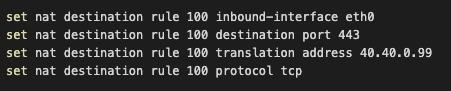
\includegraphics[width=0.9\textwidth]{Images/R2 configuration to allow traffic from eth0 to web vpn.png}
  \caption{R2 config }
  \label{fig }
\end{figure}

\subsection{Now let us try, if our administrator can connect from pc1 by, starting a VPN client with vpnclient start on it.}
In this session we connect tp PC1 and try to start vpn client on it by using the command 
\begin{itemize}
\item vpnclient start
\item vpncmd
\end{itemize}
\begin{figure}[H]
\centering
  \includegraphics[width=0.9\textwidth]{Images/Connecting VPN client on pc1 .png}
  \caption{Starting vpn client on PC1 }
  \label{fig }
\end{figure}
After connecting vpn client on pc1 we choose Management of VPN Client
\subsubsection{(a and b) We add a virtual interface called intern and create an account for the user ktr, which connects to web vpn via r2.
}
In this session after we connect to VPN client on pc1 and we enter into vpncmd, now we have to add a virtual interface called intern, we can do this by following commands.
\begin{itemize}
\item NicCreate
\item Virtual Network Adapter Name: intern
\end{itemize}
\begin{figure}[H]
\centering
  \includegraphics[width=0.9\textwidth]{Images/Adding a virtual interface called intern .png}
  \caption{Adding a virtual interface called intern }
  \label{fig }
\end{figure}

\subsection{create an account for the user ktr, which connects to web vpn via r2}
In this session we create a account for the user ktr which connects to web vpn via r2, for thatwe use the following commands.
\begin{itemize}
\item VPN Client>AccountCreate
\item Name of VPN Connection Setting: intern
\end{itemize}

\begin{figure}[H]
\centering
  \includegraphics[width=0.9\textwidth]{Images/creating an account for ktr.png}
  \caption{Creating an account for ktr}
  \label{fig }
\end{figure}


\subsection{If the connection succeeds, we can add a private IP address to the newly created NIC vpn intern, which connects to the network}
In this session we add a private IP address to the newly created NIC vpn intern which connects to the network
\begin{itemize}
\item Destination VPN Server Host Name and Port Number: 30.30.0.2:443
\item Destination Virtual Hub Name:VPN
\item Connecting User Name: ktr
\item Used Virtual Network Adapter Name: intern
\end{itemize}

\begin{figure}[H]
\centering
  \includegraphics[width=0.9\textwidth]{Images/Adding private IP .png}
  \caption{add a private IP address to the newly created NIC vpn intern}
  \label{fig }
\end{figure}

\subsection{On PC1 we start a trace-route to any web server of CD D and confirm that our target is only one hop away.
}
Now we try trace route to any of the web server of CD d and confirm that our target is only one hop away.
we use the following command to do that 
\begin{itemize}
    \item trace-route 40.40.0.100
\end{itemize}

\begin{figure}[H]
\centering
  \includegraphics[width=0.9\textwidth]{Images/Traceroute to websheldon.png}
  \caption{Trace-route to web sheldon}
  \label{fig }
\end{figure}

\section {SoftEther Cascade Connections}
VPN cascading is multi VPN connection.A further advantage of the cascade is that we can enable every web server
to communicate with each other. So if we would replace our simple web servers with
enhanced applications, which may consist of several microservices, they could securely
communicate and use the ressources of both sites. within VPN connection.
\begin{figure}[H]
\centering
  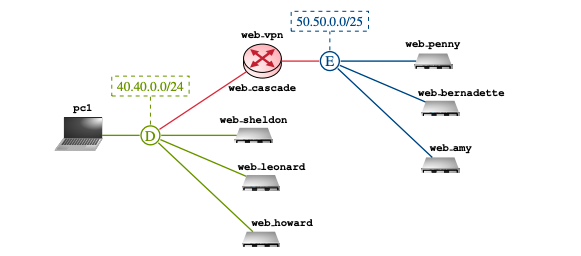
\includegraphics[width=0.9\textwidth]{Images/cascade_topology.png}
  \caption{Topology appearance after a connection to the site-to-site VPN is established}
  \label{fig }
\end{figure}

\begin{itemize}
    \item Finally, we connect both server farms over a site-to-site (s2s) VPN with a cascade connection. Our administrator can connect to both sites over a single VPN connection and reach all nodes  without any restrictions. 
\end{itemize}
\subsection{create a Softether server, called web cascade}
\begin{itemize}
    \item web cascade is created as machine in the network.
\end{itemize}
\begin{figure}[H]
\centering
  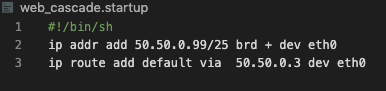
\includegraphics[width=0.9\textwidth]{Images/web_cascade.startup.png}
  \caption{Web Cascade startup file}
  \label{fig }
\end{figure}
\subsubsection{1. start the web cascade}
\begin{itemize}
    \item vpnserver start
\end{itemize}
\begin{itemize}
    \item vpncmd
\end{itemize}
\begin{figure}[H]
\centering
  
\includegraphics[width=0.9\textwidth]{Images/web_cascade start.png}
  \caption{Start the Web cascade }
  \label{fig }
\end{figure}
\subsubsection{2.Create a Hub}
\begin{itemize}
    \item HubCreate
\end{itemize}
\begin{figure}[H]
\centering
  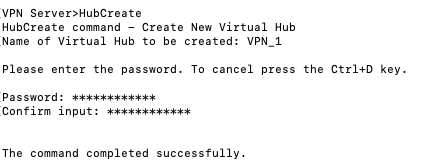
\includegraphics[width=0.9\textwidth]{Images/Hubcreate.png}
  \caption{Start the Web cascade }
  \label{fig }
\end{figure}
\subsubsection{3.On the created hub we add a cascade, which connects to the remote hub
on web vpn with the credentials of s2s.}
\begin{itemize}
    \item CascadeCreate
\end{itemize}
\begin{figure}[H]
\centering
  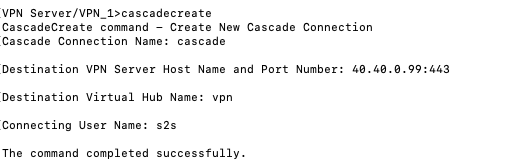
\includegraphics[width=1\textwidth]{Images/cascade_create.png}
  \caption{Create Cascade Connection }
  \label{fig }
\end{figure}
\subsection{After the configuration, a NIC tap intern was created, which needs to be
connected to eth0 by a bridge}
\subsubsection{Create a Bridge}
\begin{itemize}
    \item BridgeCreate VPN /DEVICE:intern /TAP:yes
\end{itemize}
\begin{figure}[H]
\centering
  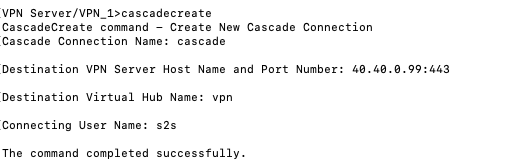
\includegraphics[width=1\textwidth]{Images/cascade_create.png}
  \caption{Create Bridge }
  \label{fig }
\end{figure}
\subsection{Additonally add a route to 40.40.0.0/24 in r2}
\begin{itemize}
    \item ip route add 40.40.0.0/24 via 30.30.0.1
\end{itemize}
\subsection{On r3 we need to modify the firewall to allow unrestricted access to web cascade}
\begin{itemize}
    \item iptables -A FORWARD -s 50.50.0.99/25  -j ACCEPT 
\end{itemize}
\begin{itemize}
    \item iptables -A FORWARD -d 50.50.0.99/25  -j ACCEPT
\end{itemize}
\subsection{If the cascade connection is established, we can add a route on web vpn to CD E}
\begin{itemize}
    \item ip route add default via  50.50.0.99 dev eth0
\end{itemize}
\subsection{Set Password for Cascade Connection}
\begin{itemize}
    \item cascadepasswordset
\end{itemize}
\begin{figure}[H]
\centering
  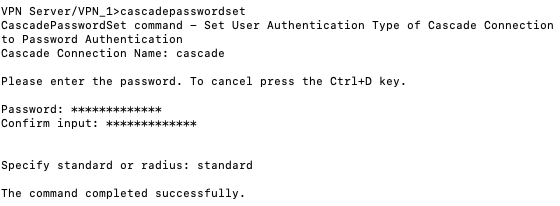
\includegraphics[width=1\textwidth]{Images/cascadepassword.png}
  \caption{Connects to the remote hub on web vpn with the credentials of s2s. }
  \label{fig }
\end{figure}
\subsection{Set the Cascade connection to online Status}
\begin{itemize}
    \item CascadeOnline
\end{itemize}
\begin{figure}[H]
\centering
  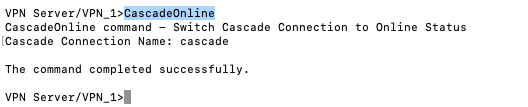
\includegraphics[width=1\textwidth]{Images/cascadeonline.png}
  \caption{Setting the status of the Cascade to online }
  \label{fig }
\end{figure}
\subsection{Within the networks being routable over the gateways web vpn and web cascade,we can setup all web servers to reach each other}
\subsubsection{1.On web sheldon, web leonard, and web howard we add a route to CD E over web vpn}
\begin{itemize}
    \item web sheldon : ip route add default via 40.40.0.99 dev eth0
\end{itemize}
\subsection{On web penny, web bernadette, and web amy we add a route to CD D
over web cascade.}
\begin{itemize}
    \item web penny : ip route add default via 50.50.0.99 dev eth0
\end{itemize}
\begin{itemize}
    \item web bernadette : ip route add default via 50.50.0.99 dev eth0
\end{itemize}
 \begin{itemize}
    \item web amy  : ip route add default via 50.50.0.99 dev eth0
\end{itemize}
\subsection{Finally for the administrator on pc1, we add a route to 50.50.0.0/25 over web vpn, which acts as a gateway for both restricted networks.}
 \begin{itemize}
    \item Web\_vpn : ip route add default via  50.50.0.99 dev eth0
\end{itemize}
\subsection{start a Curl to any web server of CD E from pc1 }
\begin{itemize}
    \item We will curl to web\_penny from Pc1(50.50.0.100)
\end{itemize}
\begin{figure}[H]
\centering
  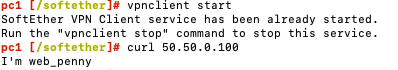
\includegraphics[width=1\textwidth]{Images/pc1 curl web penny.png}
  \caption{Curl 50.50.0.100}
  \label{fig }
\end{figure}
\subsection{start a traceroute to any web server of CD E from pc1 and
confirm that your target is only two hops away and gets routed over web\_vpn.}
\begin{itemize}
    \item traceroute 50.50.0.100
\end{itemize}
\begin{figure}[H]
\centering
  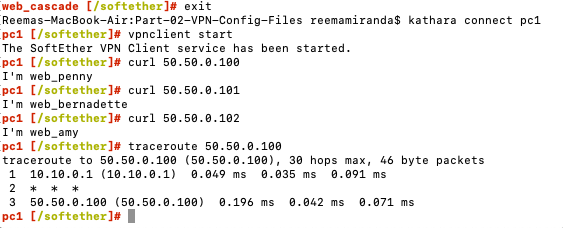
\includegraphics[width=1\textwidth]{Images/traceroute web penny.png}
  \caption{Traceroute 50.50.0.100}
  \label{fig }
\end{figure}
\begin{itemize}
    \item As we can see in the above diagram we are able to reach the webserver web\_penny (on CD E) in 2 hops.
\end{itemize}